
% Copyright (c) 2015 - 2020 Mario Mlačak, mmlacak@gmail.com
% Public Domain work, under CC0 1.0 Universal Public Domain Dedication. See LICENSING, COPYING files for details.

% Nineteen chapter ====================================================
\chapter*{Nineteen}
\addcontentsline{toc}{chapter}{Nineteen}
\label{ch:Nineteen}

\begin{flushright}
\parbox{0.8\textwidth}{
\emph{The truth is at the beginning of anything and its end are alike touching.\newline
\hspace*{\fill}{\textperiodcentered \textperiodcentered \textperiodcentered \hspace*{0.2em} Yoshida Kenko} } }
\end{flushright}

\noindent
Nineteen is chess variant which is played on 18 x 18 board, with light
gold-yellow and white fields and gold-yellow and dark gray pieces.
A new piece is introduced, Star.

\clearpage % ..........................................................
% Star ****************************************************************

\section*{Star}
\addcontentsline{toc}{section}{Star}
\label{sec:Nineteen/Star}

\vspace*{-1.0\baselineskip}
\noindent
\begin{wrapfigure}[11]{l}{0.4\textwidth}
\centering
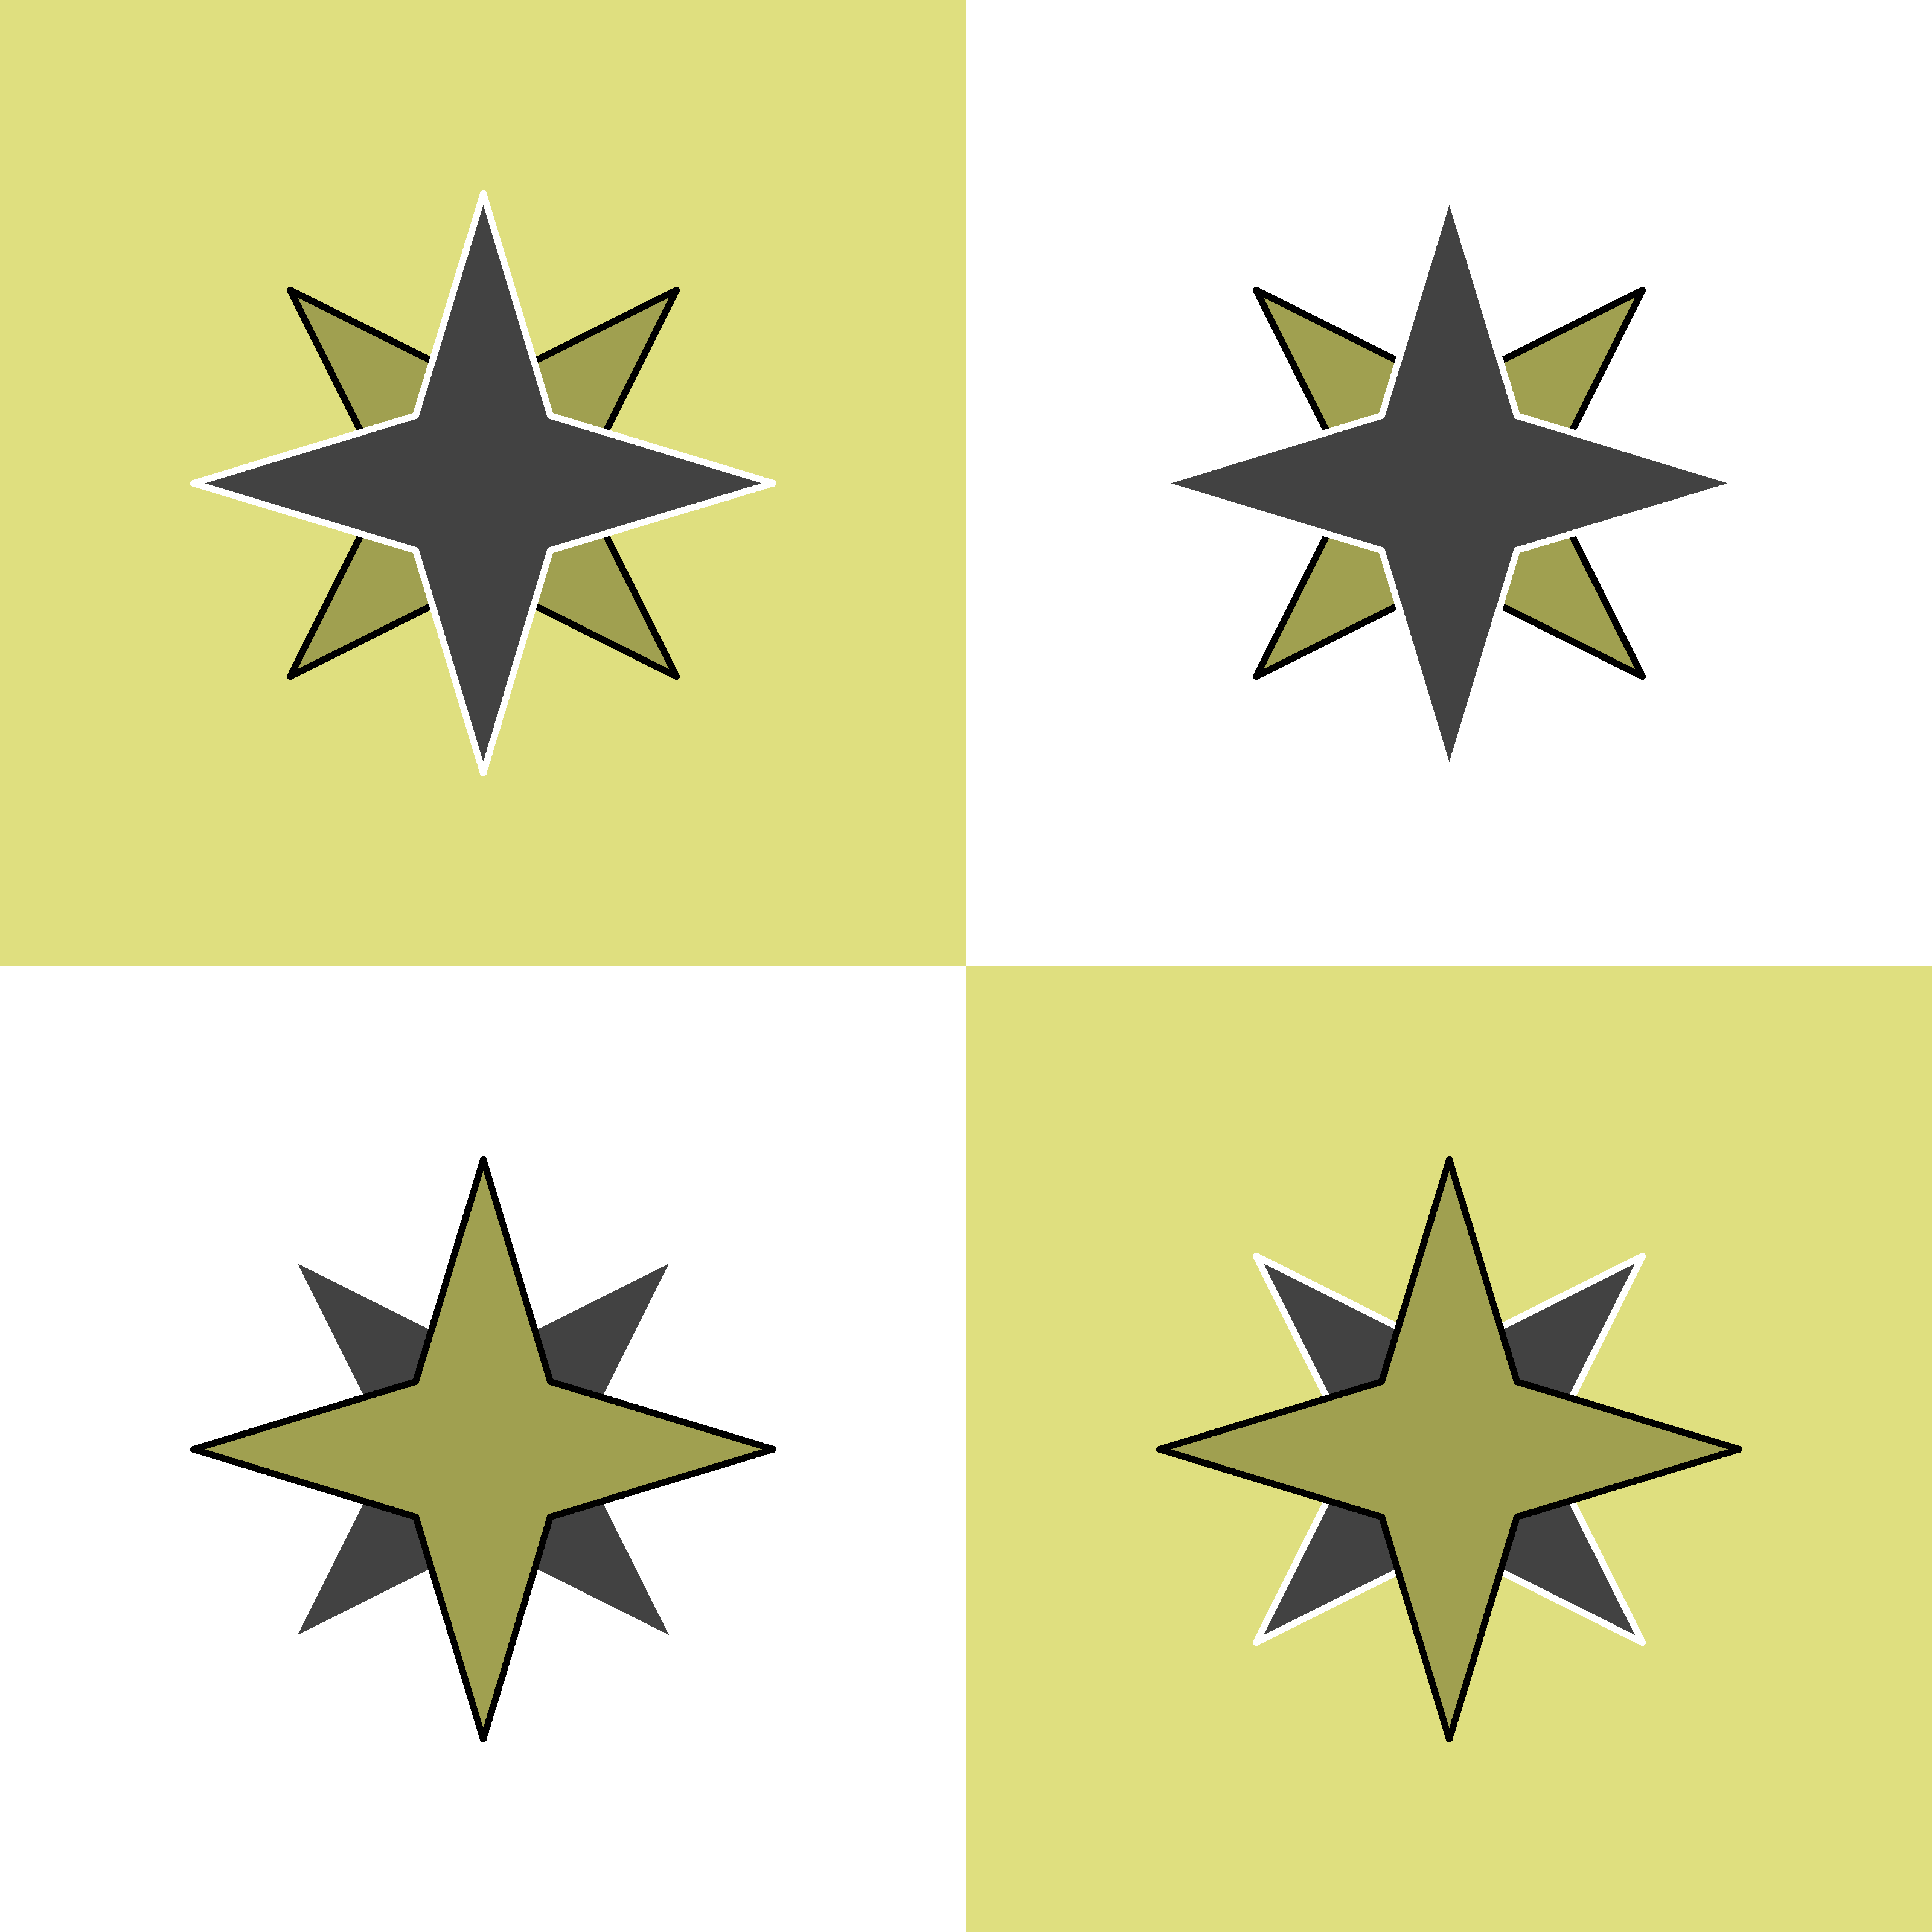
\includegraphics[width=0.4\textwidth, keepaspectratio=true]{pieces/11_star.png}
\caption{Star}
\label{fig:11_star}
\end{wrapfigure}
Star does not belong to any player, and cannot be moved, activated, captured, or
converted. Light Stars are positioned in lower left and upper right corners, dark
Stars in lower right and upper left corners.

Star is a teleporting piece. Teleportation is initiated by touching a Star, or a
field at which it stands with a piece, using either normal or capturing step. Piece
in question, if it's not Wave, then reappears on any empty portal-field near Star
in opposite color. Any momentum carried is lost, piece can't move any further from
emerging portal-field, and so a move (cascade) is finished. Teleportation is not
limited by matching colors of a piece and a Star, any piece can use any Star to
start teleporting.

Player initiating teleportation can choose which opposite color Star will be
destination, and at which empty portal-field piece will reappear. If there is no empty
portal-field near both Stars of opposite color piece is oblationed, i.e. removed from
chessboard as if it has been captured.

If teleported piece is Wave, it continues movement from a field occupied by the other
Star in the same color. Wave retains all of momentum carried into teleportation. The
way and direction of movement of Wave is the same as before teleportation.

Kings cannot be teleported. Pawns cannot be promoted to a Star.

\clearpage % ..........................................................

\subsection*{Portal-fields}
\addcontentsline{toc}{subsection}{Portal-fields}
\label{sec:Nineteen/Star/Portal-fields}

\vspace*{-1.0\baselineskip}
\noindent
\begin{figure}[!h]
\includegraphics[width=1.0\textwidth, keepaspectratio=true]{examples/12_n/scn_n_01_portal_fields.png}
\caption{Portal-fields}
\label{fig:scn_n_01_portal_fields}
\end{figure}

Portal-fields are all fields immediately surrounding a particular field
horizontally, vertically and diagonally. They are the same as step-fields
of a King.

Since all Stars are pinned into the corners of a chessboard, there are always
exactly 3 portal-fields around each one.

\clearpage % ..........................................................
% Teleporting pieces ==================================================

\subsection*{Teleporting pieces}
\addcontentsline{toc}{subsection}{Teleporting pieces}
\label{sec:Nineteen/Star/Teleporting pieces}

\vspace*{-1.5\baselineskip}
\noindent
\begin{figure}[!h]
\includegraphics[width=1.0\textwidth, keepaspectratio=true]{examples/12_n/scn_n_02_teleport_init.png}
\vspace*{-1.3\baselineskip}
\caption{Teleportation start}
\label{fig:scn_n_02_teleport_init}
\end{figure}

\vspace*{-0.5\baselineskip}
A piece (except King) can start teleporting by stepping into any Star.
Teleporting piece (if it's not Wave) can then emerge on any empty portal-field
surrounding Stars in opposite color.
Here, light Bishop is about to teleport by diving into dark Star. Portal-fields
around light Stars are numbered, Bishop could appear on any empty field. Light
Wave on field 3 blocks Bishop from emerging there, even if Wave could be activated
by Bishop in a normal, cascading move.

\clearpage % ..........................................................

\subsubsection*{Teleportation blocked}
\addcontentsline{toc}{subsubsection}{Teleportation blocked}
\label{sec:Nineteen/Star/Teleporting pieces/Teleportation blocked}

\vspace*{-1.0\baselineskip}
\noindent
\begin{figure}[!h]
\includegraphics[width=1.0\textwidth, keepaspectratio=true]{examples/12_n/scn_n_03_teleport_move_2.png}
\caption{Teleporting dark Rook}
\label{fig:scn_n_03_teleport_move_2}
\end{figure}

If all eligible portal-fields are not empty, teleported piece is blocked from
emerging, and is oblationed, i.e. removed from chessboard as if captured by
opponent.

Here, after teleportation dark Rook will be oblationed, because there is no empty
(numbered) portal-field around both Stars in opposite color.

\clearpage % ..........................................................
% Teleporting Wave ----------------------------------------------------

\subsubsection*{Teleporting Wave}
\addcontentsline{toc}{subsubsection}{Teleporting Wave}
\label{sec:Nineteen/Star/Teleporting pieces/Teleporting Wave}

\vspace*{-1.0\baselineskip}
\noindent
\begin{figure}[!h]
\includegraphics[width=1.0\textwidth, keepaspectratio=true]{examples/12_n/scn_n_04_teleport_move_3.png}
\caption{Teleporting light Wave}
\label{fig:scn_n_04_teleport_move_3}
\end{figure}

Wave can start teleporting by stepping into a Star, just like any other piece could
do. Since Wave is not obstructed by any piece on its step-fields, it can reach a Star
even if activating piece (here, Pegasus) would be blocked.

\clearpage % ..........................................................

\vspace*{-2.0\baselineskip}
\noindent
\begin{figure}[!h]
\includegraphics[width=1.0\textwidth, keepaspectratio=true]{examples/12_n/scn_n_05_teleport_end.png}
\caption{Teleportation end}
\label{fig:scn_n_05_teleport_end}
\end{figure}

Teleported Wave emerges from the other Star in the same color as the starting one.
Wave has to continue movement in the same direction as it did before teleportation,
direction cannot be changed. Wave also retains momentum it had before teleportation,
so here it can activate Pyramid, or
\hyperref[fig:scn_mv_36_activating_rush_pawn_init]{rush light Pawn for 2 fields}.

% ---------------------------------------------------- Teleporting Wave
\clearpage % ..........................................................

\subsubsection*{Teleporting Wave blocked}
\addcontentsline{toc}{subsubsection}{Teleporting Wave blocked}
\label{sec:Nineteen/Star/Teleporting pieces/Teleporting Wave blocked}

\vspace*{-1.0\baselineskip}
\noindent
\begin{figure}[!h]
\includegraphics[width=1.0\textwidth, keepaspectratio=true]{examples/12_n/scn_n_06_teleport_wave_blocked.png}
\caption{Teleported Wave blocked}
\label{fig:scn_n_06_teleport_wave_blocked}
\end{figure}

If teleported Wave has all of its step-fields blocked (here, by dark Pawns), it is
removed from chessboard, just like any other
\hyperref[fig:scn_n_03_teleport_move_2]{teleported piece which has all portal-fields blocked}.

\clearpage % ..........................................................
% Teleporting off-board -----------------------------------------------

\subsubsection*{Teleporting off-board}
\addcontentsline{toc}{subsubsection}{Teleporting off-board}
\label{sec:Nineteen/Star/Teleporting pieces/Teleporting off-board}

\vspace*{-1.3\baselineskip}
\noindent
\begin{figure}[!h]
\includegraphics[width=1.0\textwidth, keepaspectratio=true]{examples/12_n/scn_n_07_teleport_wave_init.png}
\caption{Wave out-of-board before teleportation}
\label{fig:scn_n_07_teleport_wave_init}
\end{figure}

Here, light grey fields are virtual fields extending existing chessboard.
\hyperref[fig:scn_mv_27_wave_activation_by_unicorn_first_step]{Wave activated by Unicorn}
has to choose 2 different steps at the beginning of its movement, and follow
them for the remainder of a ply. Wave's movement is legal as long as its
\hyperref[fig:scn_mv_30_wave_off_board]{ply ends on a chessboard}. So, light
Wave can reach light Star and start teleporting, even though it stepped
outside of a board.

\clearpage % ..........................................................

\vspace*{-2.0\baselineskip}
\noindent
\begin{figure}[!h]
\includegraphics[width=1.0\textwidth, keepaspectratio=true]{examples/12_n/scn_n_08_teleport_wave_end.png}
\caption{Wave teleported}
\label{fig:scn_n_08_teleport_wave_end}
\end{figure}

Teleported Wave has to continue its movement performing the same step(s) as
before teleportation. That means, teleported Wave has to continue alternating
between 2 initially chosen steps, according to a color of a current field. So,
emerging step (here, long jump) is different from a step starting teleportation
(short jump).

% ----------------------------------------------  Teleporting off-board
\clearpage % ..........................................................
% Emerging off-board --------------------------------------------------

\subsubsection*{Emerging off-board}
\addcontentsline{toc}{subsubsection}{Emerging off-board}
\label{sec:Nineteen/Star/Teleporting pieces/Emerging off-board}

\vspace*{-1.0\baselineskip}
\noindent
\begin{figure}[!h]
\includegraphics[width=1.0\textwidth, keepaspectratio=true]{examples/12_n/scn_n_09_teleport_wave_2_init.png}
\caption{Wave before teleportation}
\label{fig:scn_n_09_teleport_wave_2_init}
\end{figure}

Similar example as previous, with dark Wave which has the same steps (short,
long jump) over the same colored fields (dark, light fields) switched. So,
teleporting step is also different (here, long jump) from previous example
(short jump).

\clearpage % ..........................................................

\vspace*{-2.0\baselineskip}
\noindent
\begin{figure}[!h]
\includegraphics[width=1.0\textwidth, keepaspectratio=true]{examples/12_n/scn_n_10_teleport_wave_2_end.png}
\caption{Wave out-of-board after teleportation}
\label{fig:scn_n_10_teleport_wave_2_end}
\end{figure}

\hyperref[fig:scn_n_08_teleport_wave_end]{Again},
teleported Wave has to continue alternating between 2 initially chosen steps,
according to a color of a current field, i.e. color of starting field of each
step. Wave's movement is legal as long as its
\hyperref[fig:scn_mv_30_wave_off_board]{ply ends on a chessboard}. So, dark
Wave can e.g. activate dark Pawn (with 1 momentum carried through teleportation),
even though it stepped outside of a board.

% -------------------------------------------------- Emerging off-board
\clearpage % ..........................................................
% Teleporting Pawn ----------------------------------------------------

\subsubsection*{Teleporting Pawn}
\addcontentsline{toc}{subsubsection}{Teleporting Pawn}
\label{sec:Nineteen/Star/Teleporting pieces/Teleporting Pawn}

\vspace*{-1.4\baselineskip}
\noindent
\begin{figure}[!h]
\includegraphics[width=1.0\textwidth, keepaspectratio=true]{examples/12_n/scn_n_11_teleport_pawns_init.png}
\caption{Pawn teleporting on step-field}
\label{fig:scn_n_11_teleport_pawns_init}
\end{figure}

All pieces can access a Star on own step- or capture-field. So, light Pawn in
the same column as dark Star (here, a) can step into it, and teleport away. If
destination Star is on
\hyperref[sec:Definitions/Chessboard sides, navigation]{opponent's side of a board},
teleported Pawn is tagged for
promotion (fields 1, 2, 3). If destination portal-field is on opponent's
\hyperref[sec:Terms/Figure row]{figure row} (field 1), player can choose between
promoting Pawn outright, or keeping it tagged for promotion.

\clearpage % ..........................................................

\vspace*{-2.0\baselineskip}
\noindent
\begin{figure}[!h]
\includegraphics[width=1.0\textwidth, keepaspectratio=true]{examples/12_n/scn_n_12_teleport_pawns_step_1.png}
\caption{Pawn teleporting on capture-field}
\label{fig:scn_n_12_teleport_pawns_step_1}
\end{figure}

Pawn can also dive into a Star located at its capture-field, and teleport away.
If destination Star is on
\hyperref[sec:Definitions/Chessboard sides, navigation]{own side of a board} (portal-fields
4, 5, 6), teleported Pawn loses options to promote, and does not gain opportunity
to rush on initial move.

\clearpage % ..........................................................

\vspace*{-2.0\baselineskip}
\noindent
\begin{figure}[!h]
\includegraphics[width=1.0\textwidth, keepaspectratio=true]{examples/12_n/scn_n_13_teleport_pawns_end.png}
\caption{Pawn teleporting end}
\label{fig:scn_n_13_teleport_pawns_end}
\end{figure}

Light Pawn teleported onto own side of chessboard cannot rush, even if
destination field is on own \hyperref[sec:Terms/Pawn row]{Pawn row}. This
is so even if said Pawn is activated with more than 1 momentum, on its
initial move.

% ---------------------------------------------------- Teleporting Pawn
\clearpage % ..........................................................

\subsubsection*{Teleporting Bishop}
\addcontentsline{toc}{subsubsection}{Teleporting Bishop}
\label{sec:Nineteen/Star/Teleporting pieces/Teleporting Bishop}

\vspace*{-1.4\baselineskip}
\noindent
\begin{figure}[!h]
\includegraphics[width=1.0\textwidth, keepaspectratio=true]{examples/12_n/scn_n_14_teleport_bishop.png}
\caption{Bishop teleportation}
\label{fig:scn_n_14_teleport_bishop}
\end{figure}

Teleporting Bishop, like any other piece, can choose any empty portal-field
around opposite-color Star as a destination, regardless of a color of that
emerging field. Teleporting to a field in a different color changes (color of)
accessible fields for teleported Bishop, for the remainder of a game. Here,
such color-changing portal-fields are enumerated, 1 and 2.

\clearpage % ..........................................................

\subsubsection*{King cannot teleport}
\addcontentsline{toc}{subsubsection}{King cannot teleport}
\label{sec:Nineteen/Star/Teleporting pieces/King cannot teleport}

\vspace*{-1.4\baselineskip}
\noindent
\begin{figure}[!h]
\includegraphics[width=1.0\textwidth, keepaspectratio=true]{examples/12_n/scn_n_15_king_cannot_teleport.png}
\caption{King cannot teleport}
\label{fig:scn_n_15_king_cannot_teleport}
\end{figure}

King cannot teleport at all; regardless if positioned on own or opponent's side
of a chessboard, regardless if using Star of a matching or opposite color.

% ================================================== Teleporting pieces
% **************************************************************** Star
\clearpage % ..........................................................
% Sideways Pawns ******************************************************

\section*{Sideways Pawns}
\addcontentsline{toc}{section}{Sideways Pawns}
\label{sec:Nineteen/Sideways Pawns}

\vspace*{-1.5\baselineskip}
\noindent
\begin{figure}[!h]
\includegraphics[width=1.0\textwidth, keepaspectratio=true]{examples/12_n/scn_n_16_sideways_pawn_init.png}
\vspace*{-1.4\baselineskip}
\caption{Sideways moving Pawn}
\label{fig:scn_n_16_sideways_pawn_init}
\end{figure}

\vspace*{-0.5\baselineskip}
In this and all subsequent variants Pawn can move sideways for one field, onto a field
immediately to its left, or to its right. Side fields are just step-fields; destination
has to be empty, or it can host own Wave.

Here, light Pawn can make one step onto empty field to the left; or it can move onto
the right step-field, and activate light Wave D, with one momentum.

\clearpage % ..........................................................

\vspace*{-2.1\baselineskip}
\noindent
\begin{figure}[!h]
\includegraphics[width=1.0\textwidth, keepaspectratio=true]{examples/12_n/scn_n_17_sideways_pawn_activated_wave.png}
\vspace*{-1.4\baselineskip}
\caption{Wave activated by sideways Pawn}
\label{fig:scn_n_17_sideways_pawn_activated_wave}
\end{figure}

\vspace*{-0.5\baselineskip}
\hyperref[fig:scn_mv_15_bishop_activating_wave]{As before}, Wave inherits all steps
from its \hyperref[sec:Terms/Activator]{activator}. Wave activated by sideways Pawn
can now move laterally in addition to
\hyperref[fig:scn_mv_22_wave_activated_by_step_pawn]{straight and diagonally forward}.
Just like Pawn's, all Wave's lateral fields are just step-fields; Wave can't activate
Pyramid located on any sideways field.\newline
\indent
Here, Wave activated by Pawn on its step-field (now "in-the-air") can activate light
Knight, light Wave E or dark Wave, but none of light Pyramids. Activated Wave cannot
change direction once it starts moving; so, light Bishop is out of reach.

\clearpage % ..........................................................
% Activating Wave -----------------------------------------------------

\subsection*{Activating Wave}
\addcontentsline{toc}{subsection}{Activating Wave}
\label{sec:Nineteen/Sideways Pawns/Activating Wave}

\vspace*{-1.4\baselineskip}
\noindent
\begin{figure}[!h]
\includegraphics[width=1.0\textwidth, keepaspectratio=true]{examples/12_n/scn_n_18_capture_pawn_init.png}
\vspace*{-1.4\baselineskip}
\caption{Pawn activating Wave on capture-field}
\label{fig:scn_n_18_capture_pawn_init}
\end{figure}

\vspace*{-0.5\baselineskip}
Wave can be activated by sideways Pawn on its capture-field, with 1 momentum.
Activated Wave moves the same as if activated on Pawn's step-fields; i.e. either
forward or laterally, until the end of a chessboard.
\hyperref[fig:scn_mv_22_wave_activated_by_step_pawn]{Forward movement} is the
same as with ordinary, non-sideways Pawns, i.e. straight or diagonally forward,
towards opponent's initial positions.

\clearpage % ..........................................................

\vspace*{-2.1\baselineskip}
\noindent
\begin{figure}[!h]
\includegraphics[width=1.0\textwidth, keepaspectratio=true]{examples/12_n/scn_n_19_capture_pawn_activated_wave.png}
\vspace*{-1.4\baselineskip}
\caption{Wave activated by Pawn on capture-field}
\label{fig:scn_n_19_capture_pawn_activated_wave}
\end{figure}

\vspace*{-0.5\baselineskip}
Wave activated by sideways Pawn on its capture-field (now "in-the-air") can
activate own Pyramid only on diagonal (capture-)fields (here, light Pyramid C);
this is same as if activated by
\hyperref[fig:scn_mv_24_wave_activated_by_capture_pawn]{ordinary, non-sideways Pawn}.
Pyramids on lateral and straight forward step-fields still cannot be activated
(here, light Pyramids A and B).\newline
\indent
As before, activated Wave cannot change its direction once it starts moving;
so, light Bishop is out of reach.

\clearpage % ..........................................................
% Activating opponent's Wave ..........................................

\subsubsection*{Activating opponent's Wave}
\addcontentsline{toc}{subsubsection}{Activating opponent's Wave}
\label{sec:Nineteen/Sideways Pawns/Activating Wave/Activating opponent's Wave}

\vspace*{-1.4\baselineskip}
\noindent
\begin{figure}[!h]
\includegraphics[width=1.0\textwidth, keepaspectratio=true]{examples/12_n/scn_n_20_activating_opponents_wave.png}
\vspace*{-1.4\baselineskip}
\caption{Activating opponent's Wave}
\label{fig:scn_n_20_activating_opponents_wave}
\end{figure}

\vspace*{-0.5\baselineskip}
...

\TODO :: ADD :: example: light Wave activated by dark Pawn --> inherited steps vs. capture-steps

\clearpage % ..........................................................

\vspace*{-2.1\baselineskip}
\noindent
\begin{figure}[!h]
\includegraphics[width=1.0\textwidth, keepaspectratio=true]{examples/12_n/scn_n_21_activated_opponents_wave.png}
\vspace*{-1.4\baselineskip}
\caption{Opponent's Wave activated}
\label{fig:scn_n_21_activated_opponents_wave}
\end{figure}

\vspace*{-0.5\baselineskip}
...

\TODO :: ADD :: example: light Wave activated by dark Pawn --> inherited steps vs. capture-steps

% .......................................... Activating opponent's Wave
% ----------------------------------------------------- Activating Wave
\clearpage % ..........................................................
% Activating Pyramid --------------------------------------------------

\subsection*{Activating Pyramid}
\addcontentsline{toc}{subsection}{Activating Pyramid}
\label{sec:Nineteen/Sideways Pawns/Activating Pyramid}

\vspace*{-1.4\baselineskip}
\noindent
\begin{figure}[!h]
\includegraphics[width=1.0\textwidth, keepaspectratio=true]{examples/12_n/scn_n_20_sideways_pawn_does_not_activate_pyramid.png}
\vspace*{-1.3\baselineskip}
\caption{Pyramid can't be activated}
\label{fig:scn_n_20_sideways_pawn_does_not_activate_pyramid}
\end{figure}

\vspace*{-0.3\baselineskip}
Image above and the next one both have two examples presented in parallel, on the
top, and to the bottom.

Pawn
\hyperref[fig:scn_mv_38_activating_pyramid_by_pawn]{cannot activate Pyramid on its step-fields},
only on capture-fields.
Since side fields are also step-fields, Pyramid can't be activated by a sideways
moving Pawn, neither directly (top) nor indirectly (bottom), regardless how many
Waves where used for indirection.

\clearpage % ..........................................................

\vspace*{-2.1\baselineskip}
\noindent
\begin{figure}[!h]
\includegraphics[width=1.0\textwidth, keepaspectratio=true]{examples/12_n/scn_n_21_sideways_pawns_cascade_pyramids.png}
\caption{Pyramids cascaded by sideways Pawns}
\label{fig:scn_n_21_sideways_pawns_cascade_pyramids}
\end{figure}

Similarly
\hyperref[fig:scn_mv_39_activating_pyramid_cascade_pawn]{to previous example},
Pyramid can be activated if last active piece is not step-field moving Pawn, even
if cascade contains one.

Here, both cascades contain step-field moving Pawns, but last active pieces in both
cases are Bishops. Both Bishops can activate Pyramids, regardless if it's directly
(bottom), or indirectly, via Wave (top).

% -------------------------------------------------- Activating Pyramid
% ****************************************************** Sideways Pawns
\clearpage % ..........................................................

\section*{Pawn ranks, rows}
\addcontentsline{toc}{section}{Pawn ranks, rows}
\label{sec:Nineteen/Pawn ranks, rows}

\vspace*{-1.1\baselineskip}
\noindent
\begin{figure}[!h]
\includegraphics[width=1.0\textwidth, keepaspectratio=true]{examples/12_n/scn_n_23_pawn_ranks.png}
\caption{Pawn rows}
\label{fig:scn_n_23_pawn_ranks}
\end{figure}

In this variant, an additional rank of light (blue arrow) and dark (red) Pawns has
been added to \hyperref[fig:12_nineteen]{initial setup}. Ranks of Pawns are enumerated
starting with one closest to opponent; the closest rank being the first one (blue,
red arrows), while the standard rank of Pawns is the second rank (green, grey).

\clearpage % ..........................................................

\section*{Rush, en passant}
\addcontentsline{toc}{section}{Rush, en passant}
\label{sec:Nineteen/Rush, en passant}

\vspace*{-0.3\baselineskip}
\noindent
\begin{wrapfigure}[14]{l}{0.4\textwidth}
\centering
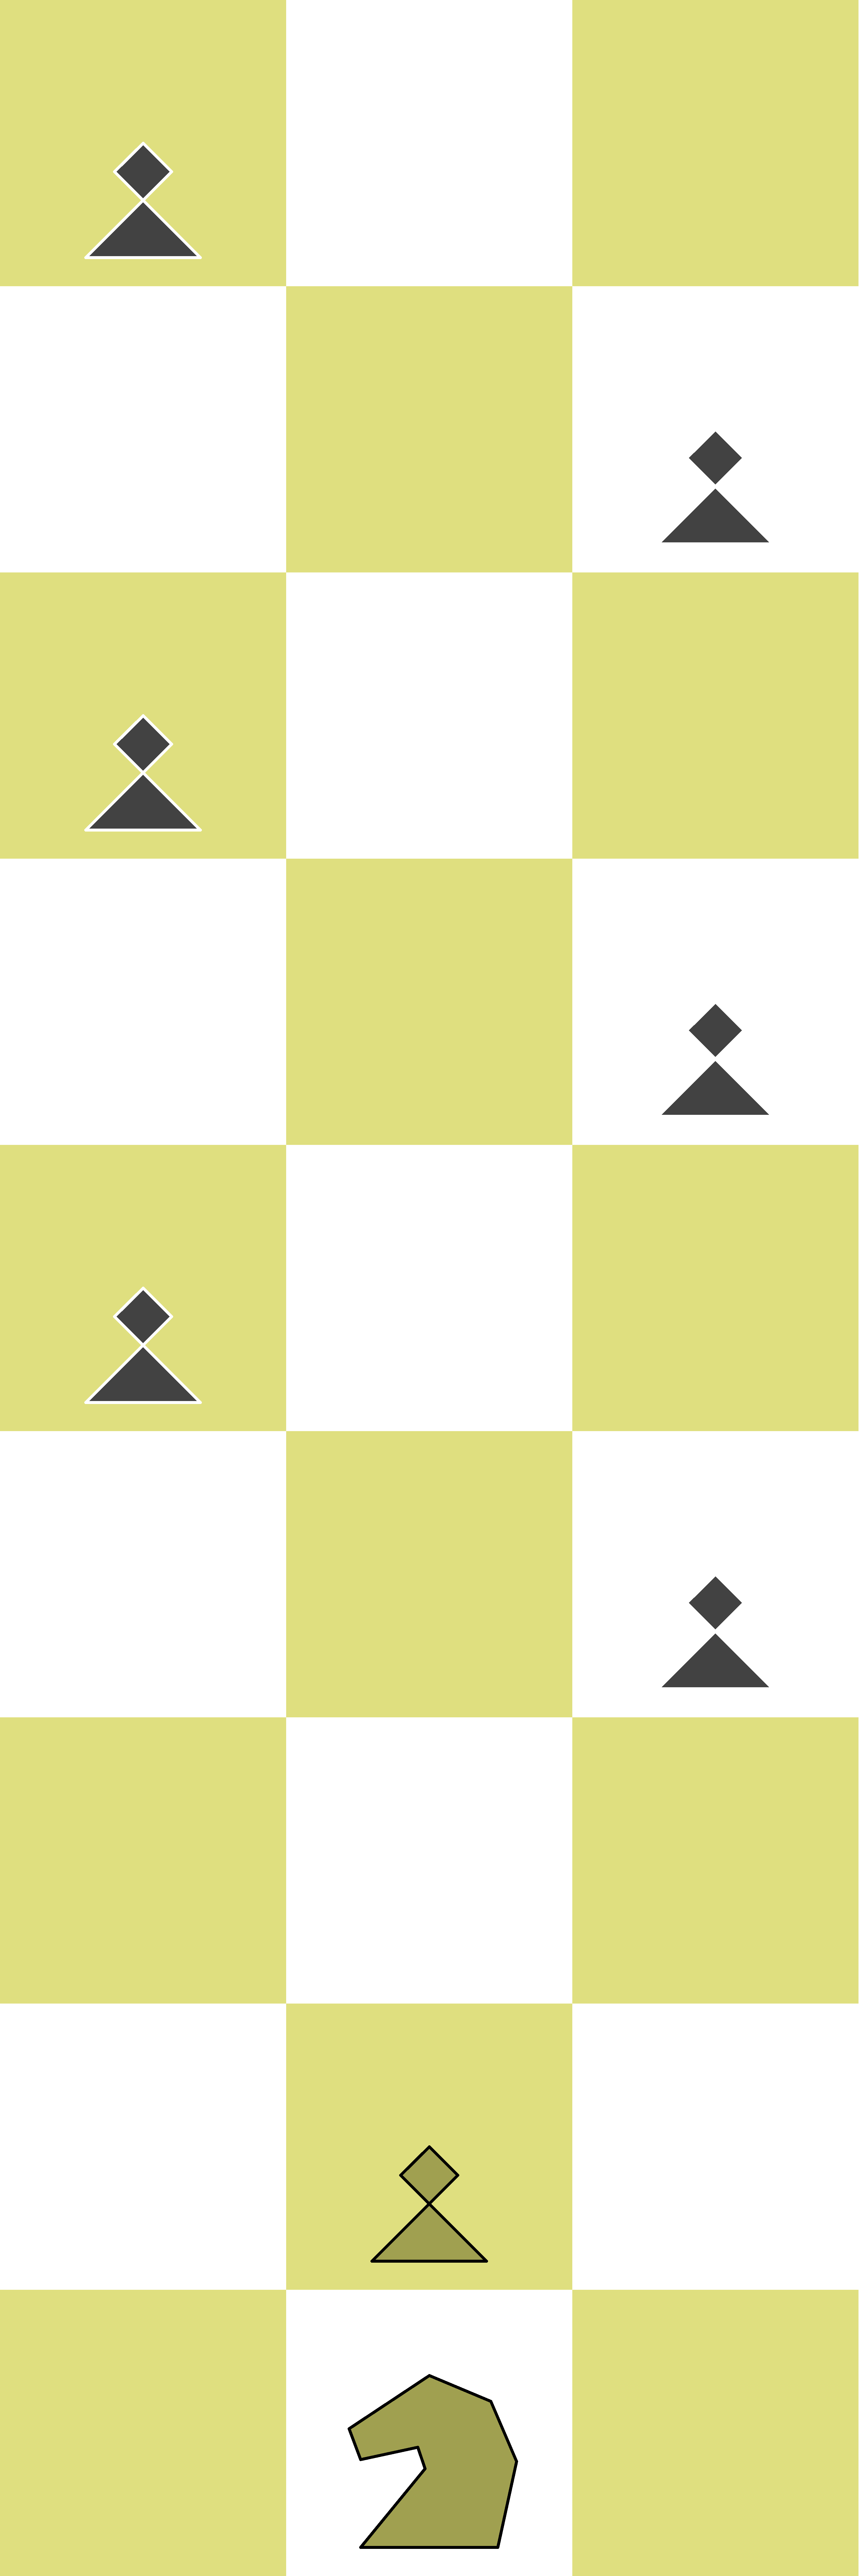
\includegraphics[width=0.4\textwidth, keepaspectratio=true]{en_passants/12_nineteen_en_passant.png}
\caption{En passant}
\label{fig:12_nineteen_en_passant}
\end{wrapfigure}
Image here have two examples presented in parallel: on the left, and to the right.

Rush and en passant are very similar to those in Classic Chess.\newline
\indent
Pawns from both ranks can be rushed, up to the other end of
\hyperref[sec:Definitions/Chessboard sides, navigation]{own side of the chessboard}.\newline
\indent
In this variant, Pawns in the first row (here, light Pawn A) can be rushed for up
to 6 fields, while those in second row (here, light Pawn B) can go up to 7 fields
forward.

% \clearpage % ..........................................................

% \TODO :: fix lmodern

\vspace*{-0.9\baselineskip}
\noindent
\section*{Promotion}
\addcontentsline{toc}{section}{Promotion}
\label{sec:Nineteen/Promotion}

Promotion is non enforced, delayed variety, i.e. it's the same as in
\hyperref[sec:Age of Aquarius/Promotion]{previous chess variant}, Age of Aquarius.

Again, Pawns cannot be promoted to a Star.

Additionally, promotion in this variant is monogamous.
Only one Queen in the same color can be present on chessboard at any given time.

\clearpage % ..........................................................

\subsection*{Only one Queen}
\addcontentsline{toc}{subsection}{Only one Queen}
\label{sec:Nineteen/Sideways Pawns/Only one Queen}

\vspace*{-1.1\baselineskip}
\noindent
\begin{figure}[!h]
\includegraphics[width=1.0\textwidth, keepaspectratio=true]{examples/12_n/scn_n_24_only_one_queen.png}
\caption{Not converting a Queen}
\label{fig:scn_n_24_only_one_queen}
\end{figure}

Opponent's Queen
\hyperref[sec:Mayan Ascendancy/Pyramid/Conversion]{can be converted as usual},
if there is no own Queen present on a chessboard, e.g. if it was captured.
In this variant, each player can have at most one Queen. If own Queen is on
a chessboard, opponent's Queen cannot be converted, and has to be captured
instead.

\clearpage % ..........................................................

\section*{Castling}
\addcontentsline{toc}{section}{Castling}
\label{sec:Nineteen/Castling}

\vspace*{-1.7\baselineskip}
\noindent
\begin{figure}[!h]
\includegraphics[width=1.0\textwidth, keepaspectratio=true]{examples/12_n/scn_n_25_new_castling_init.png}
\vspace*{-1.4\baselineskip}
\caption{New castling start}
\label{fig:scn_n_25_new_castling_init}
\end{figure}

\vspace*{-0.7\baselineskip}
In this, and all subsequent variants King is allowed to castle over attacked fields
(here, field 3), and even if it's being in check (field K).

\vspace*{-0.7\baselineskip}
\noindent
\begin{figure}[!h]
\includegraphics[width=1.0\textwidth, keepaspectratio=true]{examples/12_n/scn_n_26_new_castling_end.png}
\vspace*{-1.4\baselineskip}
\caption{New castling end}
\label{fig:scn_n_26_new_castling_end}
\end{figure}

\vspace*{-0.7\baselineskip}
All other constraints from Classical Chess remains the same; namely, King and Rook
can only castle on their first move, King cannot end its movement on attacked field,
there must be no opaque pieces between castling King and Rook. %\newline
% \indent
Since \hyperref[fig:scn_mv_07_wave_is_transparent]{it's transparent}, Wave can be
positioned between castling pieces and their destination fields.
Wave cannot be activated by castling pieces, so Wave cannot be positioned
\hyperref[fig:scn_mv_11_wave_block_castling_rook]{onto their destination field}.

\vspace*{-0.7\baselineskip}
\noindent
\begin{figure}[!h]
\includegraphics[width=1.0\textwidth, keepaspectratio=true]{castlings/12_n/nineteen_castling.png}
\vspace*{-1.4\baselineskip}
\caption{Castling}
\label{fig:nineteen_castling}
\end{figure}

\vspace*{-0.7\baselineskip}
Newly introduced
\hyperref[sec:Mayan Ascendancy/Pyramid/Conversion/Converting Rooks]{constraint from Mayan Ascendancy}
still holds, i.e. converted opponent's Rook cannot be castled, even if converted on
an initial position of own Rook. Additional difference in this variant is that King
can castle between 2 and 6 fields across.

\clearpage % ..........................................................

\section*{Initial setup}
\addcontentsline{toc}{section}{Initial setup}
\label{sec:Nineteen/Initial setup}

Stars are positioned in very corners of chessboard, light Stars in lower left and upper right
corners, dark Stars in lower right and upper left corners. Additional rank of light and dark
Pawns has been added. All other figures are also repositioned.

\noindent
\begin{figure}[h]
\includegraphics[width=1.0\textwidth, keepaspectratio=true]{boards/12_nineteen.png}
\caption{Nineteen board}
\label{fig:12_nineteen}
\end{figure}

\clearpage % ..........................................................
% ==================================================== Nineteen chapter
